% !TeX spellcheck = en_US
%*******************************************************************************
%****************************** Fourth Chapter *********************************
%*******************************************************************************
\chapter{System Implementation}
\label{chapter5}
% **************************** Define Graphics Path **************************
\ifpdf
\graphicspath{{Chapter5/Figs/Raster/}{Chapter5/Figs/PDF/}{Chapter5/Figs/}}
\else
\graphicspath{{Chapter5/Figs/Vector/}{Chapter5/Figs/}}
\fi

\section{Hardware Setup}

Teo is a quite complex system composed by sets of controllers, serial devices, sensors and actuators. It is powered by a lead-acid battery that provide nominal 12V using six series-connected cells.
The hearth of the robot is the Arduino Mega, a microprocessor that analyze the flow of data coming from all the sensors in order to define what the actuators have to do. For this reason, each component of Teo is someway(directly or not) connected to Arduino Mega. Accelerometer and capacitive sensors are in charge to detect and classify touches, they are the only components that are not directly connected to Arduino Mega. In the starter project they should have been, but the way capacitives define their value, require excessive execution time, affecting the performance of overall the system. So we needed to add an extra controller, an Arduino Nano, that processes the data coming from the capacitives and the accelerometer, telling to the main processor where the robot has been touched and how.
In this section we will talk about general Teo's hardware architecture, giving a description of the controller and the list of serial devices, sensors and actuators that are included in the project and how they are connected each other. Details about each hardware component will be discussed in the next sessions, where each Teo's functionality will be analyzed.

\subsection{Arduino Mega}
Arduino is an open-source electronics prototyping platform, designed to make the process of using electronics in multidisciplinary projects more accessible\cite{arduino:intro}. 
It consists of a physical programmable circuit board with an Atmel AVR processor and on-board I/O support; and a piece of software, or IDE (Integrated Development Environment) that runs on a computer in order to write and upload the code.
Unlike most previous programmable circuit boards, the Arduino does not need a separate piece of hardware (called a programmer) in order to load new code onto the board, it can be done just using an USB cable.The Arduino IDE uses a simplified version of C++, making it easier to learn and program.\\
The project began in Ivrea, Italy in 2005 from Massimo Banzi and David Cuartielles.
The name Arduino comes from a bar in Ivrea, Italy, where some of the founders of the project used to meet. The bar was named after Arduin of Ivrea, who was the margrave of the March of Ivrea and King of Italy from 1002 to 1014\cite{lahart2014taking}.\\
There are several Arduino boards, that differs for number of analog and digital I/O pins, processor and memory.
In this project we used an Arduino Mega as controller of the overall system. It has 54 digital input/output pins (of which 15 can be used as PWM outputs and 6 can be used to attach interrupts), 16 analog inputs, 4 UARTs (hardware serial ports), a 16 MHz crystal oscillator, a USB connection, a power jack, an ICSP header, and a reset button\cite{arduino:mega}.\\
As shown in \ref{megaConnections}, each component of the system, except to capacitive sensors and accelerometer, is connected to the Arduino Mega that, based on the senors values(inputs) and the robot state, defines what the actuators(outputs) have to do.
\begin{figure}[h]
	\centering
	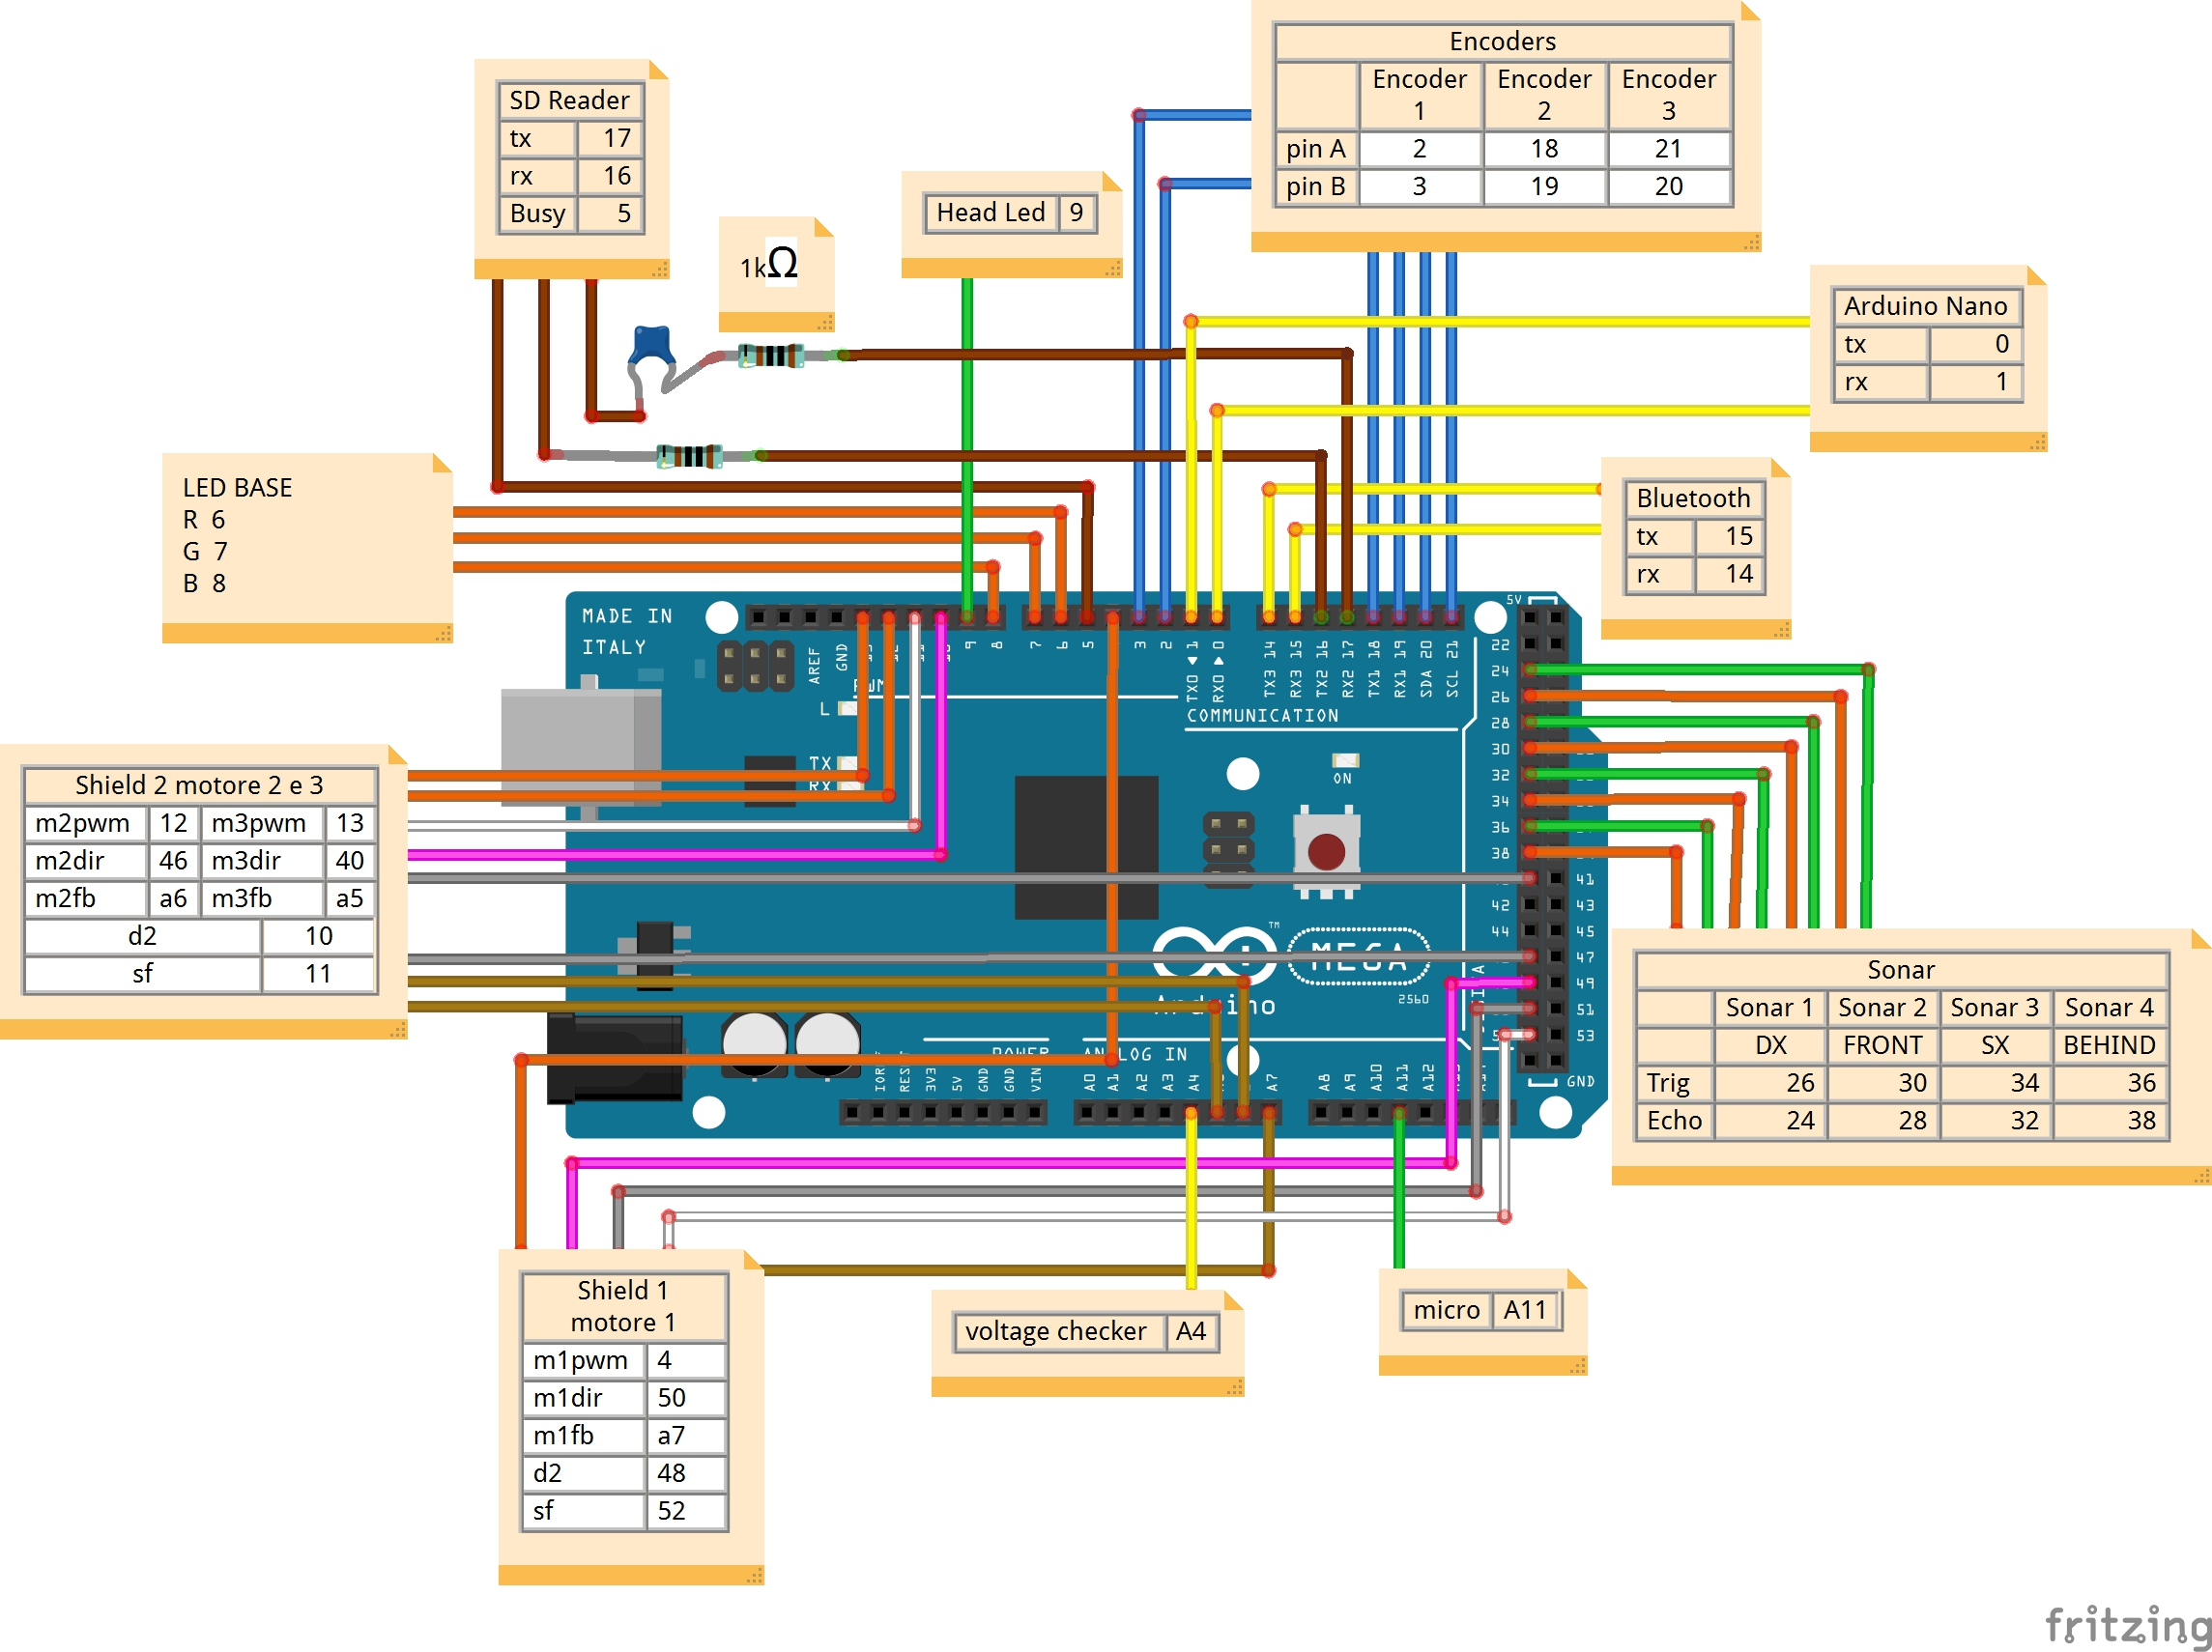
\includegraphics[width=1\textwidth]{TeoG2_bb}
	\caption{Arduino Mega connections}
	\label{megaConnections}
\end{figure}
\subsection{Serial Devices}
Arduino Mega has four UART(Universal Asynchronous Receiver/Transmitter) ports. Unlike Parallel interfaces that needs a lot of wires to transmit data, serial interfaces stream the data, sending one single bit per clock, so these interfaces can operate using only two wires: one receiver(RX), and one transmitter(TX). For this propose, Arduino Mega has eight dedicated pins.
In this project we used three Serial ports, so six pins, in the following table are listed the utilized ports, and for each one the RX and TX pin, and which device is connected to.
\begin{table}[h]
	\centering
	\begin{tabular}{|l|l|l|l|}
		\hline
		\multicolumn{1}{|c|}{\multirow{2}{*}{\textbf{\begin{tabular}[c]{@{}c@{}}Serial\\ Number\end{tabular}}}} & \multicolumn{2}{c|}{\textbf{Pin}} & \multicolumn{1}{c|}{\multirow{2}{*}{\textbf{\begin{tabular}[c]{@{}c@{}}Connected\\ Device\end{tabular}}}} \\ \cline{2-3}
		\multicolumn{1}{|c|}{} & \textbf{TX} & \textbf{RX} & \multicolumn{1}{c|}{} \\ \hline \hline
		Serial 0 & 1 & 0 & Arduino Nano \\ \hline
		Serial 2 & 16 & 17 & DF Player \\ \hline
		Serial 3 & 14 & 15 & HC-05 Bluetooth Module \\ \hline
	\end{tabular}
	\caption{Serials connections}
	\label{tab:Serials}
\end{table}\\
Looking the table its immediately evident that Serial 1 has not been included. that's because it is accessible by pin 18 and 19 that have, besides to 'serial' communication, dedicated hardware also for manage interrupts, which are necessary to guarantee an adequate functioning of the encoders. In sect.\ref{encoder} will be better discussed why interrupts are useful for the encoders.
So we were forced to use Serial 0 for the communication with Arduino Nano. Serial 0, on pin 0 and 1, uses the same UART port used by USB connection during a software update and, if both are connected, there's an obvious interference that makes mandatory to physically disconnect the serial port wires and restart Arduino. In addition to the possibility that this is rather boring, it can also cause breakdowns or loss of time when forget to disconnect the cables. But it was the last serial port available, so our choice was mandatory.
\\\\





\subsection{Sensors}
%\subsection{HC-SR04}
Teo is equipped by a lot of sensors:
\begin{itemize}
	\item four ultrasonic ranging modules(HC-SR04)
	\item one microphone sensor(Sunfounder Sound Sensor)
	\item seven capacitive sensors
	\item one accelerometer(MPU6050)
	\item three 30:1 Metal Gearmotor 37Dx68L mm with 64 CPR Encoder
	\item one battery level checker
\end{itemize}







\subsection{Actuators}
To make interaction possible and attractive, Teo has been equipped by different actuators:
\begin{itemize}
	\item two Pololu Dual MC33926 Motor Driver Shield for Arduino
	\item two speakers connected to the DFPlayer(see \ref{DFPlayer})
	\item one non addressable RGB LED strip
	\item one addressable Adafruit NeoPixel RGB Led Strip
\end{itemize}
\section{Bluetooth Connection}
Using Bluetooth Connection, a tablet or a smartphone that run Teo's application can be connected to the robot in order to send instruction and receive data. To make the connection, a blueooth module has been connected to the Arduino Mega(see \ref{tab:Serials}) and different states have been created in order to manage the instructions received and the data to send during the robot's different phases of use. 

\subsection{Bluetooth Module(HC-05)}
HC-05 is one of the most popular and cheapest module used for RF communications. It has ten meters range and allows to transform the Serial port of the Arduino Mega in a Bluetooth port, generally with a SPP(Serial Port Profile), thus becoming a serial over Bluetooth. 

\begin{figure}[h]
	\centering
	\begin{subfigure}[b]{0.4\textwidth}
		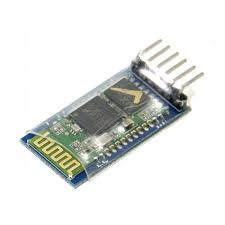
\includegraphics[width=4cm]{hc05-1}
	\end{subfigure}
	\begin{subfigure}[b]{0.4\textwidth}
		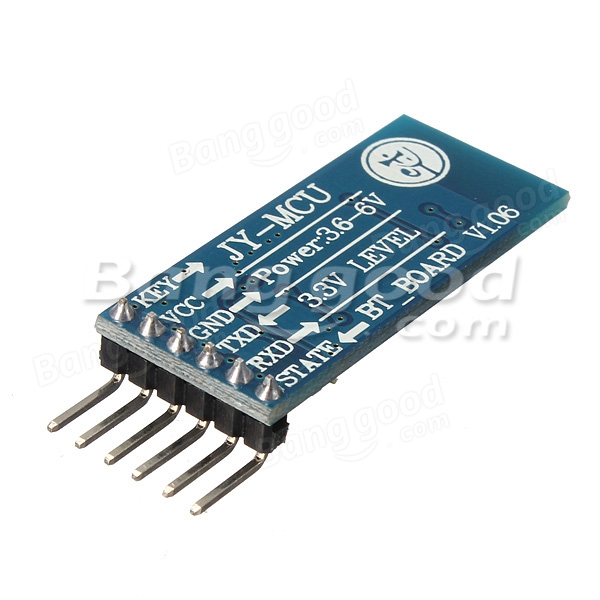
\includegraphics[width=4cm]{hc05-2}
	\end{subfigure}
	\rule{35em}{0.5pt}
	\caption{HC-05 Bluetooth Module}
	\label{HC-05}
\end{figure}
As show in \ref{HC-05}, the module has six pins, but we used only four of them: two for the power,VCC and GND connected respectively to Arduino's 5V and GND pins, and two for the serial communication(see fig.\ref{megaConnections}).
In order to work, it's important to keep in mind that the RX pin of the Arduino must be connected to the TX pin of the Bluetooth module, and, in the same way, the TX pin of the Arduino must be connected to Bluetooth RX pin.
The module can be easily set up with AT commands defining name, password, bound rate, modality(slave or master) and more.
In tab.\ref{ATCommands} it's possible to have a look on main HC-05 AT commands.
In this project, it is set with a 38400 baud rate and slave modality: the master will be the phone or tablet that will connects to it.
\\
\begin{table}[]
	\centering
	\begin{tabular}{|l|l|}
		\hline
		\textbf{Command} & \textbf{Description} \\
		\hline
		\hline
		AT & AT interface connection test \\
		\hline
		AT+RESET & Component restart \\
		\hline
		AT+ORGL & Restore to default settings \\
		\hline
		AT+ADDR? & Get module address \\
		\hline
		AT+NAME? & Get module name \\
		AT+NAME=<param> & Set module name equal to "param" \\
		\hline
		AT+ROLE? & Get module role(0=Slave/1=Master) \\
		AT+ROLE=<param> & Set module role to "param"(0=Slave/1=Master) \\
		\hline
		AT+PSWD? & Get PIN code \\
		AT+PSWD=<param> & Set PIN code equal to "param" \\
		\hline
		AT+UART? & Get Serial parameters \\
		AT+UART=<param1>,<param2>,<param3> & Set Serial parameters \\
		& (param1: Baud, param2: Stop bit, param3: Parity)\\
		\hline
	\end{tabular}
	\caption{AT Commands List}
	\label{ATCommands}
\end{table}
\subsection{Communication states}
The application presents different pages with different commands, based on the selected modality. Each page available in the App has a corresponding state on Arduino. In order to navigate between the different pages, once a choice has been made, the application sends via serial port a character that is interpreted by Arduino and define the new state and, consequently, the new page. 
Blueooth states are:
\begin{itemize}
	\item \textbf{chooseModality}: this is the initial state. It waits that the user choose between Familiarization Modality and Game Modality.
	\item \textbf{chooseGame}: once Game Modality has been chosen, this state is activated. This waits that the user choose which game will be performed.
	\item \textbf{chooseScenarioFamMod}: once a game has been chosen, one of the available scenario must be selected. This state waits that selection.
	\item \textbf{sgWaiting}: After the selection of the scenario, the application shows which patches put on which capacitive and invites to press a start button when the positioning is done. This state wait that the start button is touched.
	\item \textbf{gameModality}: when game is definitively started, the robot will act autonosmly so no one command will be send from the application until the end of the game. This state is active during all game session and when game finish it sends game data and  automatically turn to chooseModality state.
	\item \textbf{famModality}: if during chooseModality state 'Familiarization Modality' is chosen, famModality state is activated. During this state it is possible sends a lot of commands to Arduino(see \ref{FamMod}) and it also sends sensors data, with the aim to inform if sensors are working correctly.
	\item \textbf{discharge}: If battery is discharged when Teo is started up, the bluetooth state switch to discharge. In this state is impossible to give any instruction to the robot that must be charged.
\end{itemize}



\section{Basic Robot's movement control}
One important characteristic of Teo is the ability to freely move in the environment. As many others robots developed in AIRlab, Teo can move using Triskar base. It is composed by a set of 3 omni-directional wheels, each one driven by an independent gearmotor and equipped by an encoder. Two motor shield are used for control direction and power of gearmotors. This set of hardware, with an appropriate interpretation of data by software, permits to have a controlled movement of the robot, defining speed, direction and knowing at each moment where the robot is respect to its initial position. This makes also possible to create movement patterns that the robot can perform autonomously.
\subsection{Triskar base}
Triskar base is an hexagonal metal plate with 15cm of radio. Three wheels of 7cm diameter with connections at L of 4 cm length are fixed at 3 sides of the hexagon so, at \ang{120} of distance each other.
A three wheel design offers greater traction as any reactive force is distributed through only three points and the robot is well balanced even on uneven terrain. This design also reduces an additional wheel compared to a 4 wheeled robot which makes it cost effective (omni
wheels are expensive). Omnidirectional wheels, better explained in the above section, make Teo able to have an Holonomic Drive: it means that the robot has three controllable degrees of freedom and so, can always translate, rotate or both in any direction, avoiding to do any maneuver.
\subsubsection{Omnidirectional Wheels}
Omnidirectional wheels have passive rollers attached around the circumference of the center wheel which are perpendicular to the turning direction. The effect is that the robot can move in any direction and wheels  exhibit low resistance also when the movement is perpendicular to the wheel, because it can slide laterally with great ease.
\begin{figure}[h]
	\centering
	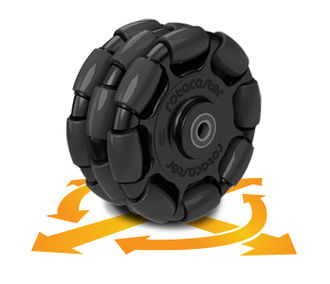
\includegraphics[width=0.3\textwidth]{omniwheel}
	\caption{Omni-directional Wheel}
	\label{fig:omniWheel}
\end{figure}
\subsubsection{Gearmotor with Encoder}
\label{encoder}
This gearmotor is a powerful 12V brushed DC motor with a 30:1 metal gearbox and an integrated quadrature encoder that provides a resolution of 64 counts per revolution of the motor shaft, which corresponds to 1920 counts per revolution of the gearbox’s output shaft. These units have a 0.61"-long, 6 mm-diameter D-shaped output shaft\cite{encoders}.\\
\begin{figure}[h]
	\centering
	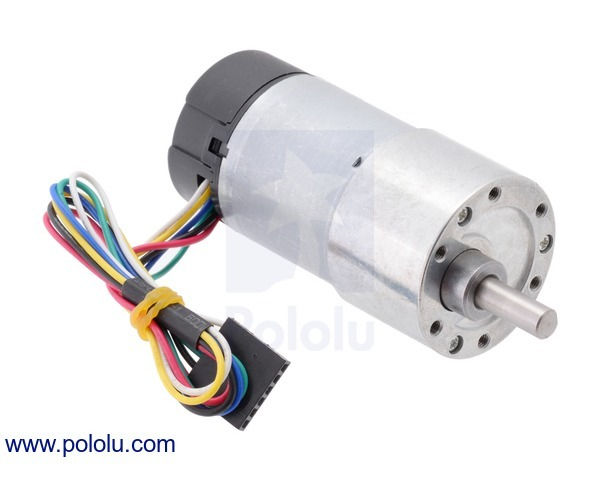
\includegraphics[width=0.5\textwidth]{gearmotor}
	\caption{Metal Gearmotor 37Dx68L mm 30:1 with 64 CPR Encoder}
	\label{fig:gearmotor}
\end{figure}
Incremental rotary encoders are widely used due to their low cost and the ability to provide signals about how much turns the gearmotor has done that can be easily interpreted and used to calculate a lot of data about Teo movement like position, orientation, speed of each wheel and of the entire robot. These data are reliable only in the presence of a floor that guarantees pure rolling motion($v=0$, $\omega\neq0$) to the wheel avoiding tangent slips and this, unfortunately, is only ideal and in reality means a loss of precision in function on the adhesion coefficient of the floor. Teo will work in indoor where it's hard to find and impervious or irregular floor and being a social robot, his movement doesn't have to be strictly precise. For this reason these encoders results as a good choice for have a feedback about Teo's movements.\\In order to work, quadrature encoders contain a code disk that is composed by two tracks, usually denoted as Channel A and Channel B. These tracks or channels are coded ninety electrical degrees out of phase, as indicated in the image \ref{fig:quad_enc_phase}, and this is the key design element that will provide the quadrature encoder its functionality.
\begin{figure}[h]
	\centering
	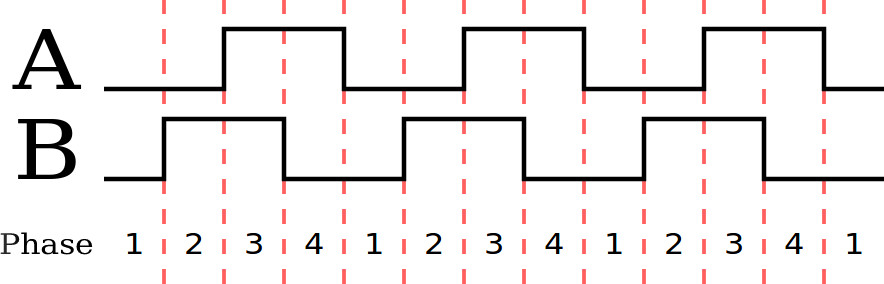
\includegraphics[width=0.8\textwidth]{encoder}
	\caption{Square waves in quadrature (clockwise rotation).}
	\label{fig:quad_enc_phase}
\end{figure}
\\
As illustrated in the fig.\ref{fig:quad_enc_phase}, when the quadrature encoder is rotating in a clockwise direction its signal will show Channel A reach the value of Channel B with one phase delay, and the reverse will happen when the quadrature encoder rotates counterclockwise.

Knowing direction, also position can be monitored. Each time one of the two channels changes its value, a counter EncCounter is incremented(clockwise rotation) or decremented(counterclockwise) based on the direction. The encoder mounted on our motor, has 1920 counts per revolution so, we can map the counter EncCounter to a degree position value and, knowing the radio R of the wheel(equals to 16cm), to a linear position value.
$$radPos= \frac{EncCounter\times2\pi}{1920}$$
$$linearPos= radPos\times R$$
Knowing the position of each wheel, speed can be derived and using inverse kinematic, is possible to define which is the real movement of the robot(look PID chapter).\\

Each gearmotor has six pins, 2 connected to the 12V battery positive and negative terminals, 2 inputs connected to Pololu Dual MC33926 Motor Driver Shield from which comes the commands  that allow motor to turn, and 2 encoder outputs(channels A and B)  connected to Arduino Mega external interrupt pins. Arduino Mega has six pins(2,3,18,19,20,21) that are able to attach interrupts and that is exactly the number of pins needed with three encoders. These pins can be set to trigger a function when the input signal is RISING or FALLING. The triggers are interpreted by hardware, so the interrupt is very fast. 
This project is full of devices that needs to work always in parallel and, being interrupts able to making things happen automatically and with maximum priority when it is needed, use them for the encoders is useful to insure that a pulse will never be missed, allowing Arduino Mega keep to manage also the other components.

\subsubsection{Pololu Dual MC33926 Motor Driver Shield}
This motor driver shield make it easy to control two bidirectional, brushed DC motors. Teo has two of them, in order to control its three wheels. As can be seen in fig.\ref{fig:dualmcscheme}, it is composed by two side, the logic one, connected to Arduino Mega, and the motor one, connected to gear motors.
\begin{figure}[h]
	\centering
	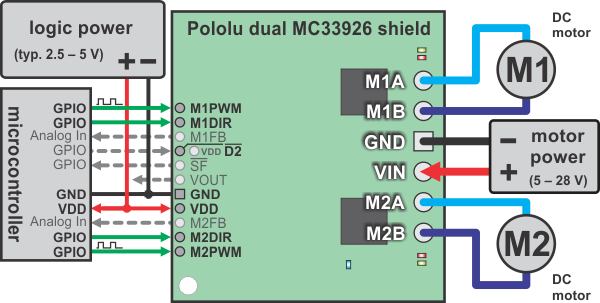
\includegraphics[width=0.6\textwidth]{dualmc21}
	\caption{Motor Driver Shield Scheme}
	\label{fig:dualmcscheme}
\end{figure}
On logic side there are VCC and GND pins for 5V power, D2 pin used to enable or disable motor driver outputs, and one PWM and DIR pin for each motor M1 and M2. The PWM pin define the power and DIR the direction of the motor. It's important to connect PWM pins on one of the fifteen Arduino PWM pins.\\
Pulse Width Modulation, or PWM, is a technique for getting analog results with digital means. Digital control is used to create a signal switched between on and off. This on-off pattern can simulate voltages between 5 and 0 Volts by changing the portion of the time the signal spends on versus the time that the signal spends off. The duration of "on time" is called the pulse width. Modifying the pulse width different analog values are obtained.\\
On motor side there are VIN and GND pins for 12V power and two pins that, based on PWM and DIR values on logic level, give the right voltage to gearmotors making them turn.
\subsection{PID}
\subsection{Inverse Kinematic}
\subsection{Direct Kinematic}
\subsection{Odometry}
\subsection{Movement Patterns}
\section{Sonars Management}
\subsection{Ultrasonic Ranging Modules(HC-SR04)}
To maintain a safer distance from the obstacles, three ultrasonic sensors are implemented on the front side and one on the back. HC-SR04 provides stable and accurate distance measurements from 2 to 400cm, with a focus of 15 degrees and a ranging accuracy that can reach up to 2mm.

Like bats and dolphins do, this sensor measures distance using ultrasonic sound that has such a high pitch that humans cannot hear. This particular sensor sends out an ultrasonic sound that has a frequency of about 40 kHz.\cite{hcsr04:datasheet}

\begin{figure}[h]
	\centering
	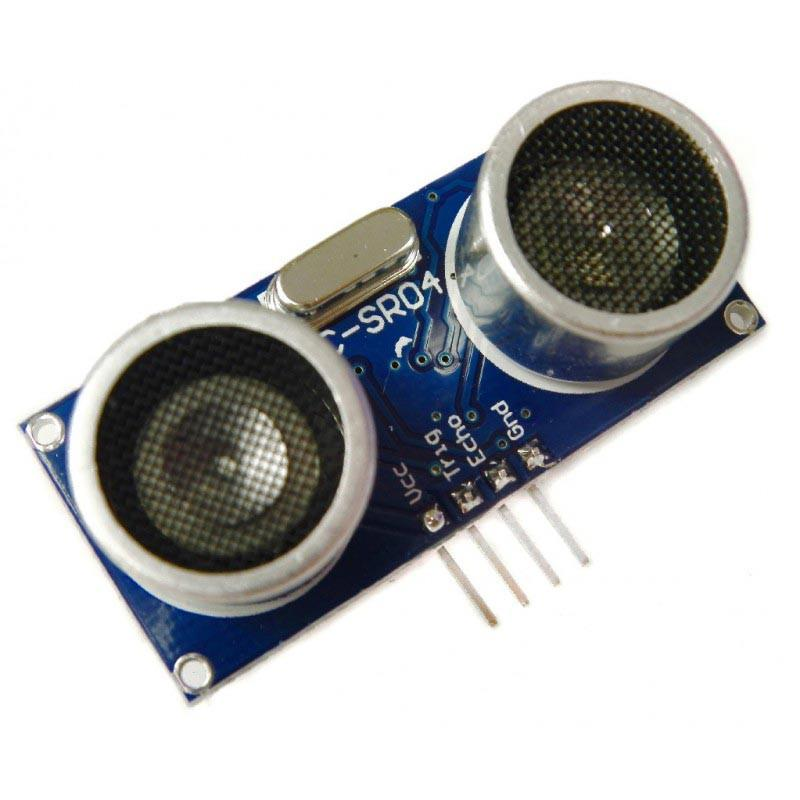
\includegraphics[width=0.3\textwidth]{hc-sr04}
	\caption{HC-SR04 module}
\end{figure}

The module is composed by an ultrasonic transmitter, a receiver and a control circuit. The transmitting phase of the sensor is called PING and it will wait for reflected signal from any obstacle in its path. This reflected signal is called ECHO. Taking trace on the time between when ping is sent and echo is received by the controller, it's possible to define the distance, using the following formula:

$$Distance = \frac{(Time \times SoundSpeed)}{2} $$

Sound travels at approximately 340 meters per second that corresponds to about 29.412µs per centimeter. The distance obtained multiplying $time\times speed$ must be divided by 2 because the signal sent from the sensor have to travel until it bounces on a surface and then return back, making the same distance two times.\\
The module has four pins: two(VCC and GND) for the power, and two(Echo and Trigger) used in order to communicate with Arduino.

DIGRESSIONE SU COME SONO MESSI I SONAR(ANGOLO DI VISUALE CON DISEGNO DEI CONI DEI TRE SONAR AFFIANCATI E IMMAGINE DEI SONAR DI TEO)
\subsection{Sonars orientation}
As you can see in picture NN, the 3 sonars on the front are oriented in order to have a 90 degrees vision. This allows Teo to have a reasonable view of the obstacles present in the environment, making it consequently able to autonomously navigate in the space.
\subsection{Input filtering and classification}
\section{Audio Playback}
\subsection{DF Player}
\label{DFPlayer}
The DFPlayer Mini MP3 Player for Arduino is a small and cheap MP3 module with an simplified output directly to the speaker. The DFPlayer perfectly integrates hard decoding module, which supports common audio formats such as MP3, WAV and WMA including 30 level adjustable volume and 6 level EQ adjustable. Besides, it also supports TF and MicroSD card with FAT16 or FAT32 file system. Thanks to this module is possible, through a simple serial port, to play any audio file, without great effort.

\begin{figure}[h]
	\centering
	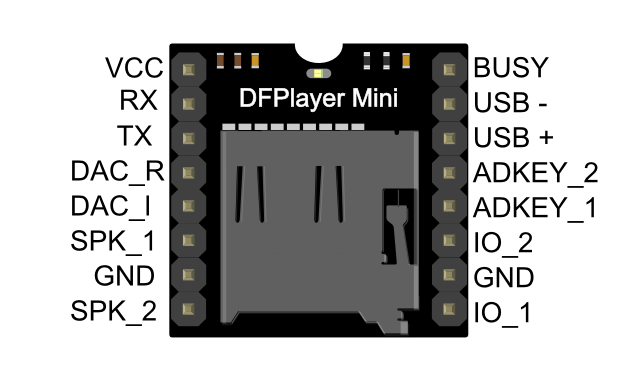
\includegraphics[width=0.6\textwidth]{dfplayer}
	\caption{DFPlayer module}
	\label{fig:DFPlayer}
\end{figure}
\subsection{Speakers}
As already talked in sec.\ref{DFPlayer}, Teo has two speakers that make it able to speak, play music and make various sounds. These are connected to the DF Player SPK\textunderscore1, SPK\textunderscore2 and ground(GND) and positioned on the bottom side of Teo, where they can be well listen but can't be reached and touched by children, avoiding they to damage them.
\subsection{Software Management}
\section{Touch Detecting}
\subsection{Arduino Nano}
The Arduino Nano is a small and complete board based on the ATmega328. It has 22 digital input/output pins (of which 6 can be used as PWM outputs), 8 analog inputs, one UART (hardware serial ports), and works with a Mini-B USB cable instead of a standard one\cite{arduino:nano}.\\
In this project the Arduino Nano is a bridge between the Arduino Mega and all the sensors(capacitives and accelerometer) that deal with detecting and classifying touches.
\begin{figure}[h]
	\centering
	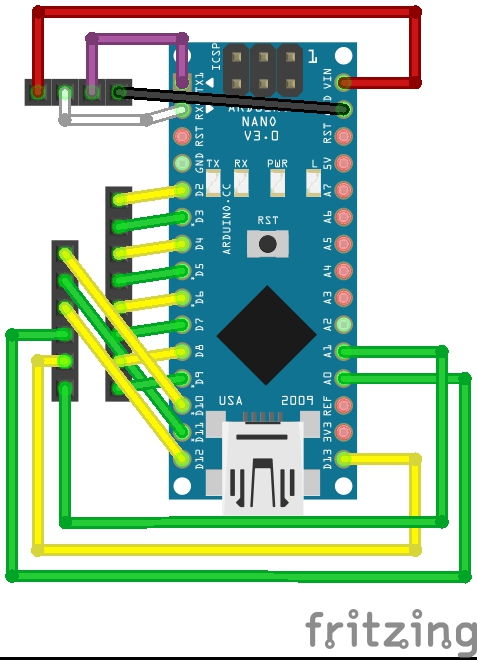
\includegraphics[width=0.4\textwidth]{arduinoMicroSchema_bb}
	\caption{Arduino Nano connections}
	\label{nanoConnections}
\end{figure}

\subsection{Communication between two Arduinos}
\subsection{Capacitive Sensors}
\begin{figure}[h]
	\centering
	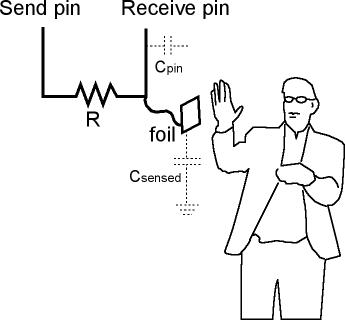
\includegraphics[width=0.3\textwidth]{CapSense}
	\caption{How Capacitive sensors work}
\end{figure}
Capacitive senors are a very important and innovative element for Teo functionalities.\\
There are seven capacitive sensors on Teo: three on the body(one on the belly, two on the back), used to detect touches and classify them in pats, hits and hugs, and four on the head, used in Game Mode in order to answer questions. 
The sensors have been completely developed by us with easy to find and cheap material, so the cost is very low. We had to try a lot of different configuration(see REF) in order to have good results. 

The setup includes an high value resistor(10MOhm) between the send pin and the receive (sensor) pin. The receive pin is the sensor terminal that, connected to a metallic net, makes the capacitive area.

When the send pin changes state, it will eventually change the state of the receive pin. The delay between the send pin changing and the receive pin changing is determined by an RC time constant, defined by $R \times C$, where R is the value of the resistor and C is the capacitance at the receive pin, plus any other capacitance (e.g. human body interaction) present at the sensor(receive) pin\cite{CapSenseLib}. Being $R$ a constant, bigger will be the capacitance means a big delay.\\

Being Teo powered by a battery, arise a ground problem for capacitors. 
-SPIEGARE MEGLIO-
attaccati al pc abbiamo un riferimento di massa invariato nel tempo, essendo la massa connessa a terra
con la batteria il riferimento di massa è variabile nel tempo, non essendo più costante, si perde stabilità ed efficienza.

mettendo la massa dietro, quando una persona tocca, la viariazione di capacità aumenta, e la massa relativa della batteria viene influenzata dalla mesa a terra del soggetto che tocca

The solution was to put another metallic net, connected by a wire to the battery ground pin, under the sensor net, insulated by a synthetic polyester wadding((FIBRA DI POLIESTERE(ovatta sintetica in poliestere)).Che isola lasciando flessibile e lasciando la possibilità di premere e deformare. This worked really well to stabilize sensor values and also seemed to efficaciously increase sensor sensitivity.

PARLARE DEL PROBLEMA DI OCCUPAZIONE DEL PROCESSORE PER TEMPO INDETERMINATO CHE HA SPINTO AD USARE UN ARDUINO EXTRA


\subsection{Accelerometer(MPU6050)}

\begin{figure}[h]
	\centering
	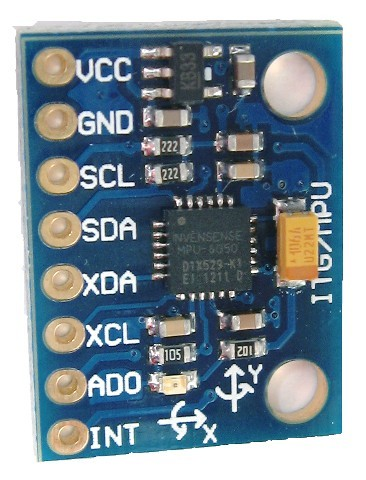
\includegraphics[width=0.2\textwidth]{mpu6050}
	\caption{MPU-6050 module}
\end{figure}


Able to capture the acceleration on the three axes, used with the capacitive sensors to define when the robot is hitten.

The MPU-6050 sensor contains a MEMS accelerometer and a MEMS gyro in a single chip. It is very accurate, as it contains three 16-bits analog to digital conversion hardware for digitizing the gyroscope outputs
and three 16-bit ADCs for the accelerometer outputs. Therefor it captures the x, y, and z channel at the same time. The sensor uses the I2C-bus to interface with the Arduino.\cite{MPU6050}

The MPU-6050 is not expensive, especially given the fact that it combines both an accelerometer and a gyro.
\subsection{Touch classification}
\subsection{Touch reactions}
\section{Micro Detecting}
\subsection{Microphone Sensor(Sunfounder Sound Sensor)}
\begin{figure}[h]
	\centering
	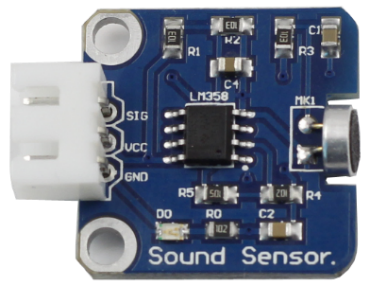
\includegraphics[width=0.3\textwidth]{soundSensor}
	\caption{Sunfounder Sound Sensor}
\end{figure}
Sound sensor is a component that receives sound waves and converts them into electrical signal. It detects the sound intensity in ambient environment converting audio signals into electrical signals. This module is used for detect high audio noise around the robot, such as screams. It has 3 pins, 2 for the power(5v), and one is the signal sensor output, connected to A11 Arduino analog-in pin. 
\subsection{Filtering and threshold}
\subsection{Reaction Behaviors}

\section{Leds Management}
\subsection{Non Addressable RGB LED Strip}
\label{LEDSTRIP}
A multicolor non addressable RGB LED strip is positioned on the bottom of Teo, just around the chassis. An RGB element is composed by three different LEDs(red, green, blue) arranged so can interact each other to form different complementary colors. Non addressable means that all strip LEDs display the same color at any time and this can be manipulated varying the voltage applied to each of the three power inputs, connected trough a MOSFET to Arduino Mega's PWM pins.


\subsection{Adafruit NeoPixel Addressable RGB LED Strip}
An Adafruit Multicolor Addressable RGB LED Strip has been placed on the head of Teo. In this LED strip, unlike the one of previous section(Sect.\ref{LEDSTRIP}),is powered by 5V and each LED has its own chip and can be individually triggered for color changing. Thanks to this, LEDs in the strip can light up in different colors at the same time \cite{schiller2010automated}.
Thanks to Adafruit library, this strip also needs an easier setup compared to the previous one, it has only one input pin directly connected to a PWM Arduino's pin and two pins for 5V power.
\subsection{Led Patterns and colors}

\section{Autonomous Movements}
\subsection{Exploring}
\subsection{Following}
\subsection{Mixed Movement}
\section{Moods Expression}
\subsection{Happy}
\subsection{Sad}
\subsection{Scared}
\subsection{Angry}

\section{Game Alghorithm}
\subsection{Data Collection}
\section{Battery Level Check}
Arduino analog inputs can be used to measure DC voltage between 0 and 5V. Teo's battery provides nominal 12V, it means it's voltage will be between 11.5V when discharged and 13.5V when fully charged. In order to measure voltages greater than 5V, two resistors have been used to create a voltage divider able to proportionally decreases the battery voltage to one within the range of the Arduino analog inputs. 

\begin{figure}[h]
	\centering
	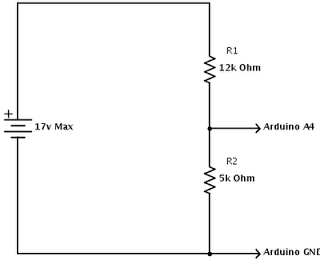
\includegraphics[width=0.5\textwidth]{voltage-divider}
	\caption{Voltage Divider Diagram}
	\label{fig:voltageDiv}
\end{figure}

With the aim to protect Arduino pins from voltages higher than 5V, we assumed an overestimated the maximum value of the battery, 17V instead of 13.5V, that is the usual voltage value of a full charged battery, and applying the voltage divider formula with the selected resistances $R1=\SI{12}{\kohm}$ and $R2=\SI{5}{\kohm}$
$$V_{out}=V_{in}\frac{R2}{R1+R2}=17V\frac{\SI{5}{\kohm}}{\SI{5}{\kohm}+\SI{12}{\kohm}}=5V$$
we can see that with $V_{in}=17V$ the voltage on Arduino Mega($V_{out}$) will be 5V. Being $V_{in}=17V$ a maximum overestimated value, we can ensure that $V_{out}$ will never exceed 5V.
The code in the Arduino Mega is in charge to recalculate the battery voltage value starting from the voltage received on the analog pin and, in case it is lower than 11.5V, Teo will warn the therapist about its need to be charged. 